\documentclass[openany]{ntuthesis}

\usepackage{times}
\usepackage{verbatim}
\usepackage{color}
\usepackage{url}
\usepackage{graphicx}
\usepackage{array}

% Using the tex-text mapping for ligatures etc.
\defaultfontfeatures{Mapping=tex-text}

% Set the default fonts
\setmainfont{Times New Roman}
\setCJKmainfont{BiauKai}

% Your information goes here
% author: Tz-Huan Huang [http://www.csie.ntu.edu.tw/~tzhuan]

% ----------------------------------------------------------------------------
% "THE CHOCOLATE-WARE LICENSE":
% Tz-Huan Huang wrote this file. As long as you retain this notice you
% can do whatever you want with this stuff. If we meet some day, and you think
% this stuff is worth it, you can buy me a chocolate in return Tz-Huan Huang
% ----------------------------------------------------------------------------

% Syntax: \var{English}{Chinese}
\university{National Taiwan University}{國立臺灣大學}
\collage{College of Electrical Engineering and Computer Science}{電機資訊學院}
\institute{Department of Computer Science and Information Engineering}{資訊工程學系}
\title{BodyTalk: Using Body Language Communication in Online Cooperative Games}{肢體談話:使用肢體語言溝通的網路合作遊戲設計}
\author{Wang, Wei-Han}{王偉翰}
\studentid{R01944015}
\advisor{Mike Y. Chen, Ph.D.}{陳彥仰 博士}
\year{2014}{103}
\month{July}{7}
\day{8}

\begin{document}

\frontmatter

\makecover

\makecertification

\begin{acknowledgementszh}
感謝實驗室的夥伴們對於我的幫助,尤其是同組的夥伴們,我們互相學習、互相加油打氣,我們一起努力的日子是我最難忘的回憶。也感謝我的指導教授陳彥仰老師,給予了我許多的建議,且十分支持我的研究。感謝所有在過程中給予我幫忙的朋友,你們的每一分付出,都成就了這篇論文的每字每句,謝謝你們。

\end{acknowledgementszh}

%\begin{acknowledgementsen}
%I'm glad to thank\ldots
%\end{acknowledgementsen}

\begin{abstractzh}

螢幕共享 (Screen Sharing) 在 PC 上已經發展很久的技術,在 PC 上有許多螢幕共享的軟體,例如: VNC 、 Windows Remote Desktop 等。在行動裝置上,也有越來越多的設備支援螢幕鏡像輸出 (Screen Mirroring) ,例如: iOS 及 Apple TV 支援 AirPlay Mirroring 、 Android 手機上支援 Miracast ,以及 Chromecast 也即將支援和 Android 的螢幕鏡像輸出。我們發現在手機的鏡像輸出串流中,因為行動裝置的視覺回饋,可能會導致新的攻擊手法,例如:按下螢幕上的虛擬鍵盤,所按的鍵會放大,以增進使用者體驗,但是若此時攻擊者能攔截到鏡像串流的畫面資料,那麼使用者的輸入資料將會完全外洩,即使是在輸入密碼時也一樣。我們針對 AirPlay Mirroring ,實作了一套的中間人攻擊 (Man-in-the-middle Attack) 程式,能自動化的截取出 iOS 設備鏡像串流中所輸入的密碼,證明確實存在此安全問題。最後,針對此攻擊,我們也提出了幾個包括系統層面,或是安全協定層面的解決方法。

\end{abstractzh}

\begin{abstracten}

The idea of sharing contents throughout different screens had been widely applied on personal computers for many years, such as the VNC, Remote Desktop and other related applications. While on mobile devices, the similar technique (a.k.a Screen Mirroring) had become more and more popular through these years. For instance, Apple had developed AirPlay Mirroring technique to stream contents from iOS devices to Apple TVs; Google also developed corresponding technique to share screen contents between Android devices and Chromecasts. Based on the observation of how users interact with such technique on real devices, we discovered a new attacking approach base on the fact that the visual feedbacks (e.g. the selected key will be highlighted when typing with virtual keyboard) on mobile devices are not well protected during the streaming process. To prove our concept, we implemented a system using man-in-the-middle attack approach to steal the secret codes when users enter them on their own devices while streaming contents to the remote screen. Finally, we provided some possible solutions to prevent the proposed attacking approach.

\end{abstracten}

\begin{comment}
\category{I2.10}{Computing Methodologies}{Artificial Intelligence --
Vision and Scene Understanding} \category{H5.3}{Information
Systems}{Information Interfaces and Presentation (HCI) -- Web-based
Interaction.}

\terms{Design, Human factors, Performance.}

\keywords{Region of interest, Visual attention model, Web-based
games, Benchmarks.}
\end{comment}


\tableofcontents
\listoffigures
\listoftables

\mainmatter

% Your thesis goes here
\chapter{Introduction}
\label{c:intro}
The Internet has enabled billions of people around the world to connect, communicate, and cooperate. However, even the most widely spoken language, Mandarin, is only spoken by 12\% of the world population. 
Other official languages of the United Nations, like English and French, are only spoken by 4.8\% and 1.0\% of the world, respectively \cite{I1}. 
Even if we include non-native speakers who are able to communicate in that language, they still only represent 12\% and 3\% of the world, respectively \cite{I2,I3}. This means that even for someone who speaks two of the most popular languages in the world, the person is only able to communicate with a small percentage of the world population.

One of the most popular activities on the Internet is playing cooperative games, with three of the top online cooperative games having sold more than 50 million copies. The Entertainment Software Association (ESA) indicated that there were 59\% Americans played video games, and 62\% of gamers played games with others \cite{I4}. To understand how language barriers affect cooperative gaming experience, we conducted a 12-person user study with three popular online cooperative games. We collected participants' experience and rating using extended Short Feedback Questionnaire (eSFQ) \cite{eSFQ} and Cooperative Performance Metrics (CPMs) \cite{CPMs}, as well as interviews. The study results showed that while none of the participants with common languages reported the gaming experience as frustrating, up to 67\% of the participants without common languages did. Also, participants without common languages rated fun and enjoyment significantly lower at 3.6 vs 4.3 on average (on a scale of 1 to 5) compared to participants with common languages. 

Because a significant portion of human communication is expressed through body language \cite{GD2}, this paper explores the effects of using body language in cooperative games for players with and without language barriers. We developed an online cooperative platform, BodyUp, that uses Microsoft Kinect sensors to capture body postures (i.e. skeletal tracking), Wii controllers to move the avatars, and microphones to capture voice and transmit these data in real-time over the Internet (as shown in Figure 1a). 

\begin{figure}[t]
\centering
\includegraphics[width=0.9\columnwidth]{Figures/Topic.pdf}
\caption{(a) Playing cooperative games with body language over the Internet, (b) Body language expression from actual BodySense gameplay.}
\label{fig:Topic}
\end{figure}

We also developed a game using the BodyUp platform, called Mute Robot, that supports cooperative gaming in three communication modes: 1) speaking only, 2) body language only, and 3) both speaking and body language. We designed Mute Robot to enable pairs of players to cooperate to solve puzzles. It consists of three asymmetric puzzle stages, where only one player can see the solution hints and needs to guide the other player to solve the puzzles. Figure 1b) shows examples of body language expression during actual gameplay.

We conducted a 48-person user study using these three communication modes, with half of the users having common languages and half without. The study results showed that adding body language to cooperative games increased the fun and enjoyment ratings for all players (both with and without common languages) from an average of 3.8 to 4.4 (on a scale of 1 to 5). 

Also, in speaking-only mode, the negative co-experience reported by players without common languages was more than 3 times than that reported by players with common languages. Adding body language improved their positive co-experience by 33\% and reduced their negative co-experience by 73\%. 

In terms of preference, 75\% of the players with common languages and 83\% of the players without common languages preferred having body language communication. Overall, 83\% of the players found having body language to be more cooperative.


\chapter{Related Work}
\label{c:related work}

Related works fall within two areas: cooperative game design, and body language.

\section{Cooperative Game Design}

Several prior works have explored and analyzed cooperative game design patterns. Zagal et al. explored cooperative patterns within board games and yielded some observations that game designers might consider useful for designing collaborative game \cite{CG1}, and it also presented an ontology with a view to analyzing game play \cite{CG3}. 
Bjork and Holopainen presented a large quantity of game design patterns \cite{CG2}, including cooperative and social interaction patterns.
Rocha et al. presented a framework of several cooperative game design patterns and analyzed the actual impact of using these game mechanics to design a cooperative video game \cite{CG4}.
El-Nasr et al. extended Rocha et al.'s model and proposed Cooperative Performance Metrics (CPMs) to evaluate game experience \cite{CPMs}.

Wolmet et al. reported a study of how parents and children play several cooperative co-located games with different characteristics \cite{CG5}. 
Mark et al. \cite{CG6} evaluated the communicative and cooperative behavior of same-age and mixed-age pairs (Young-Young, Young-Old, Old-Old), and identified noticeable difference between group types. 
Hamilton et al. \cite{CG7} explored how to design games for children to play with cerebral palsy, and it also presented several cooperative gameplay prototypes.

In our work, we explored and evaluated the possibility to use body language as a communication manner in cooperative game design, and analyzed the communication pattern with players.

\section{Body Language}

Consist of human communication, there is not only speech but also inclusive of various gestures and body motions. Body language, a non-verbal way to transmit your thoughts without verbalizing. According to The 7\% Rule\cite{GD2}, the influence of communication for verbal is only 7\% but is 93\% for non-verbal expression. And the non-varbal expression is made up of body language (55\%) and tones of voice (38\%).

Charades\cite{GD3} is a word guessing game. It is an acting game in which one player act as a word or a phrase, and sometimes imitates a similar pronounced words, while the other players guess the answer. The main idea is to use the body to make physical expression rather than using verbal language. 

Inspired by The 7\% Rule and the Charades, we suggested using body language as a communication manner in cooperative game to normalize player's communication skill. With this idea, whether players are playing with different language speakers or not, their communication skill is near enough for a game developer to design a proper difficulty to entertain players. On the other hand, many researchers have argued that the body movement brings about a positive emotional and social response \cite{GD7, GD8, GD9}. We believe that body language communication should enhance game engagement and enjoyment.

\chapter{Cross-Language Experience for Current Cooperative Games}

 To understand how language barrier affects the cooperative experience for current games, we conducted a 12-person user study where half the participants shared common languages and half did not. 

\section{Study Design}

We recruited 3 Japanese speakers and 9 Taiwanese speakers, and confirmed that none of the Taiwanese speakers understood Japanese and vice versa. 3 pairs of the participants did not have a common language (Japanese-Taiwanese) and 3 pairs did (Taiwanese).

We selected 3 popular cooperative games currently on the market that had distinct gameplay and cooperation needs. Also, all three games supported real-time voice chat. 
\begin{enumerate}
    \item Rocketbirds - Hardboiled Chicken: a cooperative action game, in which players shoot enemies with different weapons.
    
    \item Portal 2: a cooperative puzzle game, in which players can create portals that teleport players and must use them intelligently to solve the puzzles.
    
    \item Monaco: a cooperative stealth game, in which players can evade guards, collect coins, and escape.
\end{enumerate}

In order to simulate cooperative gameplay over the Internet, pairs of players were placed in two different rooms and used headsets to communicate with each other. Participants played each of the three games for 30 minutes, and filled out an eSFQ\cite{eSFQ} questionnaire after each game. We also conducted open-ended interviews to understand their gaming experience at the end of the sessions. 



\section{Results}

eSFQ\cite{eSFQ} has been widely used for rapid assessment of game experience. Players are asked to provide Likert-scale ratings (on a scale of 1 to 5) and to select multiple keywords to describe aspects of their experience. 
For this study, we focus on the fun/enjoyment ratings and the frustrating co-experience. 

\begin{figure}[!t]
\centering
\includegraphics[width=0.9\columnwidth]{Figures/PS_FunAndEnj.pdf}
\caption{The eSFQ Fun and Enjoyment rating (on a scale of 1 to 5) of three cooperative games for players \textit{with} and \textit{without} common languages.}
\label{fig:PS_FunAndEnj}
\end{figure}


\begin{figure}[!t]
\centering
\includegraphics[width=0.9\columnwidth]{Figures/PS_Frus.pdf}
\caption{The eSFQ Frustration index, which is the percentage of players who reported a frustrating experience, of three cooperative games for players \textit{with} and \textit{without} common languages.}
\label{fig:PS_Frus}
\end{figure}


Figure~\ref{fig:PS_FunAndEnj}, shows the average eSFQ Fun and Enjoyment rating for each game, for players \textit{with} and \textit{without} common languages. 
A rating of 5 is the highest level of fun and means ``Yeah, fun'', and a rating of 1 is the lowest level of fun and means ``Yawn, boring''.
The rating was lower for all three games when the players did not have common languages. Overall, the Fun and Enjoyment rating was 3.6 vs 4.3 for players without common languages compared to those who could communicate using a common spoken language.

Figure~\ref{fig:PS_Frus} shows the eSFQ Frustration index, which is the percentage of players who reported the experience as frustrating, for players \textit{with} and \textit{without} common languages.
For two out of the three games, Portal 2 and Monaco, frustration is significantly higher for players without common languages than those who did. In fact, none of the players with a common spoken languages reported any of the games as frustrating. 


\section{Discussion}

The Rocketbirds' gameplay mainly consists of dodging and shooting, and required the least communication outside the game. As player P5 commented (shown in Table 1): ``We couldn't talk to each other, but communicated through moves and jumps.'' 
None of the players reported Rocketbirds as frustrating, and language barriers had the least effect on its fun and enjoyment rating as well.

Portal 2 was reported as the most frustrating by players without common languages. Portal 2's primary gameplay is to solve complex puzzles, which requires precise collaboration between the two partners. As some of the players mentioned: ``I couldn't tell what my partner was trying to do without talking to each other.''(P5), and ``It was tiring because it was hard to express my ideas.'' (P4).

Monaco's gameplay allowed a single player to solve a challenge, although cooperation would make it significantly easier. Player P4 mentioned: ``I didn't know where the exit was, and my partner couldn't tell me.'', yet P9 stated:  ``This game is simple. We didn't really need any communication with each other.''.



\vspace{4ex}
\begin{table}[htbp]
    \centering
    \begin{tabular}{|p{100pt}|p{250pt}|}
        \hline
            Game & Feedback from Players without Common Languages\\
        \hline
        	Rocketbirds & \begin{itemize}
	 	 \item ``Although it was slower without talking, the challenges could still 
    	be beaten with patience.''(P2)
    	\item ``We couldn't talk to each other, but communicated through moves and jumps.''(P5)
	  	\end{itemize}
    	\\
        \hline
            Portal 2 & 
    	\begin{itemize}
    	\item ``It was tiring because it was hard to express my ideas.''(P4)
    	\item ``I couldn't tell what my partner was trying to do without talking to each other.''(P5)
    	\end{itemize}
    	\\
        \hline
        Monaco & 
    	\begin{itemize}
    	\item ``I didn't know where the exit was, and my partner couldn't tell me.''(P4)
    	\item ``This game is simple. We didn't really need any communication with each other.''(P9)
    	\end{itemize}
    	\\
    	\hline
    \end{tabular}
    \caption{Interview comments by players without common languages.}
  	\label{tab:table1}
\end{table}


% \begin{table}[!h]
%   \centering
%   \begin{tabular}{
%   !{\vrule width2pt}c
%   !{\vrule width2pt}p{0.7\columnwidth}
%   !{\vrule width2pt}c}
%     \hline
%     \centering\tabhead{Game} &
%     \multicolumn{1}{p{0.7\columnwidth}!{\vrule width2pt}}{\centering\tabhead{Feedback from Players without Common Languages}} \\
%     \hline
%     Rocketbirds & 
%     \begin{itemize}
% 	  \item ``Although it was slower without talking, the challenges could still 
%     be beaten with patience.''(P2)
%     \item ``We couldn't talk to each other, but communicated through moves and jumps.''(P5)
% 	  \end{itemize}
%     \\
%     \hline
%     Portal 2 & 
%     \begin{itemize}
%     \item ``It was tiring because it was hard to express my ideas.''(P4)
%     \item ``I couldn't tell what my partner was trying to do without talking to each other.''(P5)
%     \end{itemize}
%     \\
%     \hline
%     Monaco & 
%     \begin{itemize}
%     \item ``I didn't know where the exit was, and my partner couldn't tell me.''(P4)
%     \item ``This game is simple. We didn't really need any communication with each other.''(P9)
%     \end{itemize}
%     \\
%     \hline
%   \end{tabular}
%   \caption{Interview comments by players without common languages.}
%   \label{tab:table1}
% \end{table}

\chapter{BodyTalk Platform and Game Design}

\begin{figure}[!h]
\centering
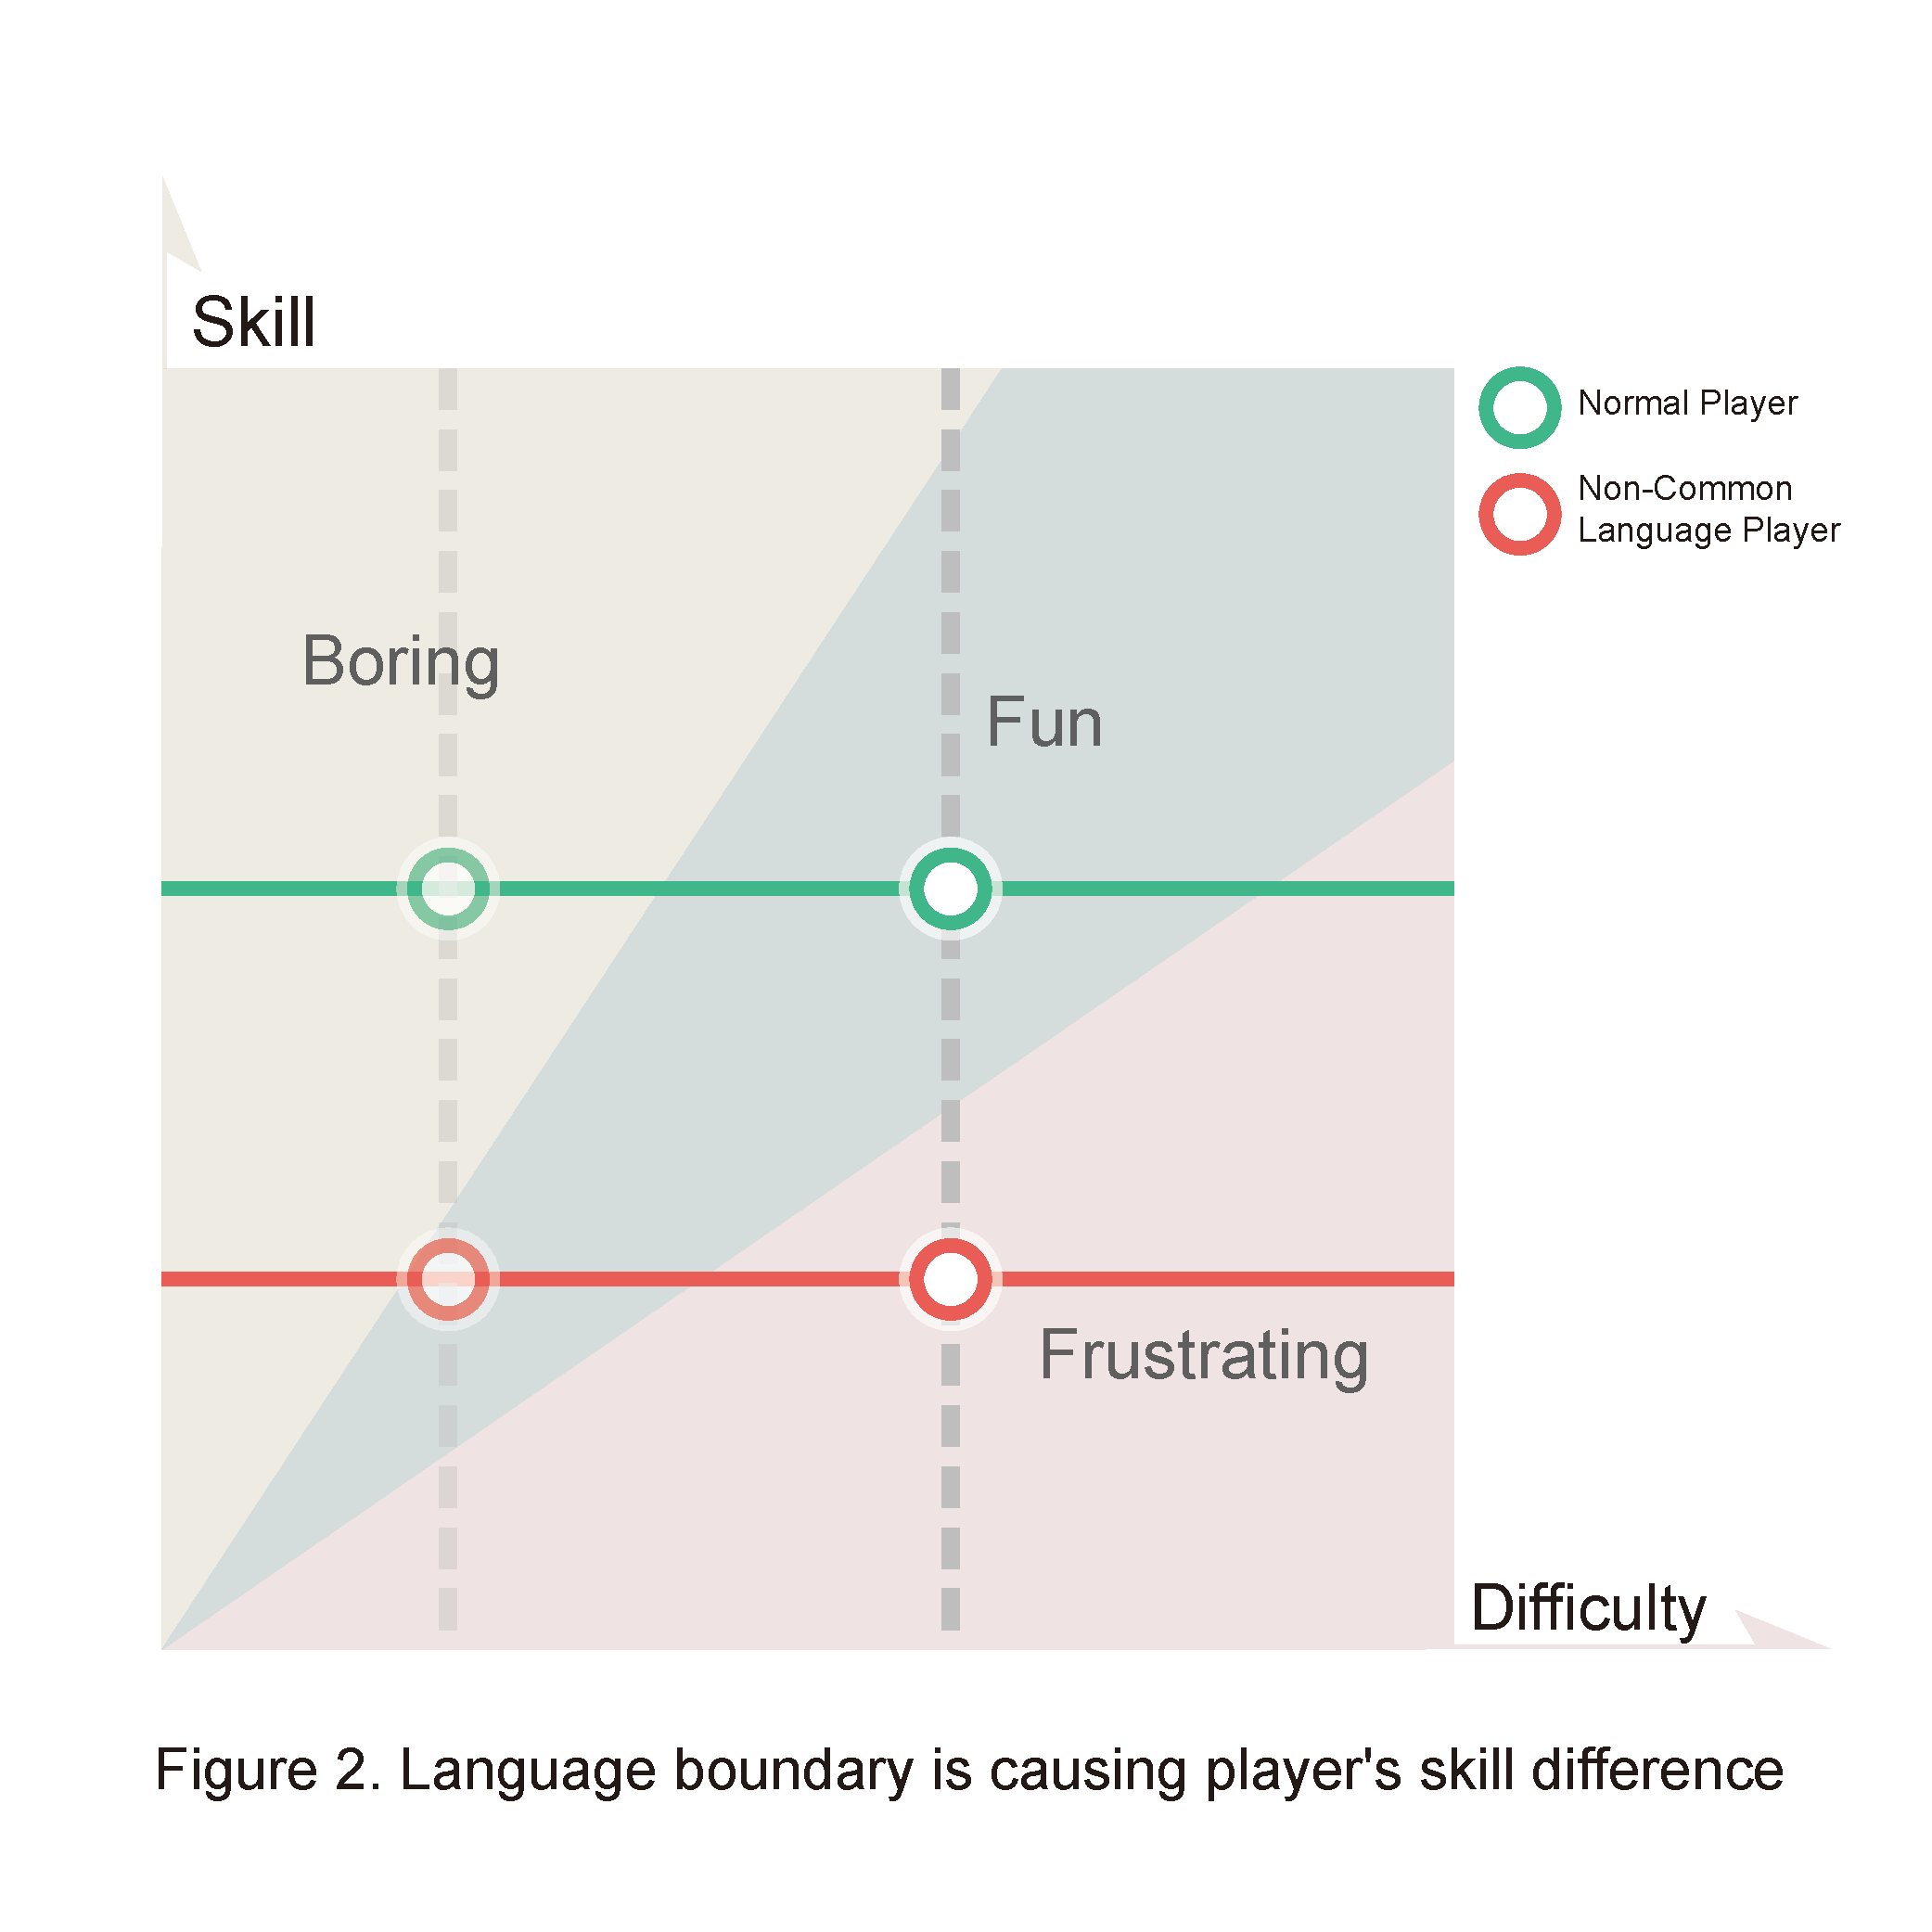
\includegraphics[width=0.9\columnwidth]{Figures/GD_F1.pdf}
\caption{Players cooperative skill levels are lower without a common language. Adding body language communication increases them, and may move the experience from being frustrating to fun.}
\label{fig:GD_F1}
\end{figure}

GameFlow\cite{GD1} discussed how game difficulty and players' skill levels affect whether players would perceive the experience as boring, fun, or frustrating. As shown Figure~\ref{fig:GD_F1}, when the difficulty is greater than the player's skills, the experience is frustrating. On the other hand, when the difficulty is less than the player's skills, the experience will be boring.



Observation from our study indicated that playing a cooperative game with a partner that did not have a common language significantly decreased players' skill level. At a difficulty level that was designed to be fun for players with common languages, that difficulty level was too challenging for players that could not communicate through languages, which lead to a frustrating experience. 

One way to solve this problem is to decrease the game's difficulty. However, this method makes the experience boring for players that had common languages. By adding body language to the gameplay, players without common languages would be able to increase their skill level, and potentially move the experience from frustrating to fun (as shown in Figure~\ref{fig:GD_F1}).  

\section{System Design and Implementation}


Our BodyTalk platform uses a Kinect depth camera (v1) and Micrsoft's Kinect SDK (v1.8) to capture each player's skeletal movement. 
Wii controller is used for navigation (e.g. move left, right, up, down) and selection (e.g. OK, Cancel). 
This combination of input modality enables users to use both arms and both legs freely for expressive body language communication.
These data are sent using Unity engine's\cite{unity} Network View over the Internet in real-time.

We developed a cooperative puzzle platformer game, called Mute Robot, using our BodyTalk platform. Two players at two distinct locations cooperate to solve a series of puzzle challenges, and their body movements are rendered as 3D avatars in real-time (see Figure~\ref{fig:GD_F3}). 


\begin{figure}[!t]
\centering
\includegraphics[width=0.9\columnwidth]{Figures/GD_F3.pdf}
\caption{Body movement mapping between player and avatar by Kinect}
\label{fig:GD_F3}
\end{figure}


\begin{figure}[!t]
\centering
\includegraphics[width=1.0\columnwidth]{Figures/GD_F2.pdf}
\caption{The asymmetric puzzle game design in one of Mute Robot's stages. (a) Bottom player's view, (b) Top player's view}
\label{fig:GD_F2}
\end{figure}


\section{Game Stage Design}


In order to have the players cooperate closely, we designed an asymmetric puzzle gameplay. The two players each sees a different view of the game with only one player receiving the hints to solve a puzzle, and must guide the other player to solve it. The roles of the hint giver and the hint receiver alternate after each stage, and the puzzles increase in difficulty. 

Figure~\ref{fig:GD_F2} shows an example of the two distinct views as seen by the two players. The left view shows the bottom player's view with the puzzle hints, and the right view shows the top player's view (which does not have the hints). 

Our prototype game has three stages. The first stage is a classic puzzle in cooperative games, where one player has to express a randomly generated secret sequence to the other player. In our design, the player must press three spatially separated buttons in the correct order to unlock a door to advance to the next stage.

The second stage, as shown in Figure~\ref{fig:GD_F2}, has a combination lock with three wheels. All three wheels must be turned to the correct selection in order the unlock the door. The first wheel's symbols are two boolean values (O and X). The second wheel's symbols are three numbers (3, 4, 7), and the last wheel's symbols are animals (fish, chicken, monkey and elephant). The set of correct symbols is randomly generated each time.

For the third stage, we wanted to explore abstract concepts. So it randomly selects one of three emotions (angry, happy and tired), for one player to pass to the other player. That player must spell the emotion correctly by selecting from a set of on-screen letters in the correct order to pass the stage.
\chapter{User Study}

Our goal is to explore how body language affects cooperative experience for players with and without common languages. 

\section{Study Design and Participants}
We set up our prototype game with three distinct communication modes: speaking only, body language only, and both speaking and body language. 


Each pair of players were placed into two separate rooms, so that they could not see nor hear each other. The rooms were on the same local area network to minimize network latency. At the beginning of each session, players practiced controlling the avatars via Kinect and Wii controllers and speaking to their partners through voice over IP (VOIP). 

Each pair of players completed all Mute Robot stages three times, each time using one of three communication modes. The order of the communication modes was counterbalanced to eliminate the effects of ordering.
Each time the players completed Mute Robot using one of the communication modes, they filled out a Short Feedback Questionnaire (eSFQ)\cite{eSFQ} questionnaire to rate their experience. 

At the end of the session, the players filled out a final questionnaire comparing their preferences, and we conducted interviews to get their qualitative feedback. Each session took about 1 hour to finish. 
In addition, all the gameplay was recorded on video and we manually coded them using Cooperative Performance Metrics (CPM)\cite{CPMs}. 

We recruited 48 participants (15 females) with average age of 22.6, for a total of 24 pairs of participants. Half of the participant pairs shared a common language (Mandarin). The other half of the pairs were ask to speak in a language that could not be understood by their partners (12 Taiwanese speakers paired with 5 Japanese, 2 German, 1 Netherlander, 1 Chilean, 1 Iraqi, 1 Russian, and 1 Guatemalan).
  


\section{Short Feedback Questionnaire (eSFQ) Results}
In our analysis, we focus on the fun/enjoyment ratings and both the positive and negative co-experience as described through the selected keywords. 


\subsection{Fun/Enjoyment Ratings}

\begin{figure}[!b]
\centering
\includegraphics[width=0.9\columnwidth]{Figures/US_Fun.pdf}
\caption{eSFQ: fun/enjoyment rating for players \textit{with} and \textit{without} common languages.}
\label{fig:US_Fun}
\end{figure}


Figure~\ref{fig:US_Fun} shows the fun/enjoyment rating for players with and without common languages using the three communication modes. 
For players with common languages, their mean rating for Speaking mode was 3.58 (SD = 1.14), and the most popular keywords selected were ``simple'' (83\% of the users) and ``intuitive'' (54\%). 
Their mean rating for Body language mode was 4.54 (SD = 0.66), and the most popular keywords selected were ``intuitive'' (54\%), ``exciting'' (46\%) and ``great'' (42\%). 
Their mean rating for Both mode was 3.96 (SD = 1.00), and the most popular keywords selected were ``intuitive'' (63\%), ``simple'' (63\%) and ``exciting'' (33\%). 

For players without common languages (see Figure~\ref{fig:US_Fun}), 
their mean rating for Speaking mode was 4.08 (SD = 0.97), and the most popular keywords selected were ``great'' (42\% of the users), ``intuitive'' (38\%), ``simple'' (38\%), and ``confusing'' (33\%). 
Their mean rating for Body language mode was 4.46 (SD = 0.66), and the most popular keywords selected were ``intuitive'' (54\%), ``exciting'' (46\%), ``simple'' (38\%) and ``difficult'' (33\%). 
Their mean rating for Both mode was 4.50 (SD = 0.59). , and the most popular keywords selected were ``intuitive'' (67\%), ``exciting'' (42\%), ``simple'' (42\%), ``great'' (34\%) and ``confusing'' (33\%).


As we can see in Figure~\ref{fig:US_Fun}, the two communication modes with body language had higher fun/enjoyment ratings compared to the speaking-only mode for all players (both with and without common languages). 



\subsection{Positive and Negative Co-experience}

\begin{figure}[!t]
\centering
\includegraphics[width=0.8\columnwidth]{Figures/US_eSFQ_Pos_Average.pdf}
\caption{eSFQ: average co-experience of positive indexes (Cooperative, Happy, Fun, Fair, Encouraging, Triumphing, Satisfying).}
\label{fig:US_eSFQ_Pos_Average}
\end{figure}

\begin{figure}[!t]
\centering
\includegraphics[width=0.8\columnwidth]{Figures/US_eSFQ_Neg_Average.pdf}
\caption{eSFQ: average co-experience of negative indexes (Defeat, Angry, Frustrating, Boring).}
\label{fig:US_eSFQ_Neg_Average}
\end{figure}


Figure~\ref{fig:US_eSFQ_Pos_Average} shows the average positive co-experience indexes for players with and without common languages. The positive co-experience is higher for communication modes with body language. Compared to speaking-only mode, adding body language 
improved positive co-experience by an average of 31\% and 33\% for players with and without common languages, respectively.

Figure~\ref{fig:US_eSFQ_Neg_Average} shows the average negative co-experience indexes for players with and without common languages. Compared to speaking-only mode, adding body language 
improved negative co-experience by an average of 13\% and 73\% for players with and without common languages, respectively.

\begin{figure}[!b]
\centering
\includegraphics[width=0.9\columnwidth]{Figures/US_Co-ex_Dif_Pos.pdf}
\caption{Positive co-experience indexes for players without common languages.}
\label{fig:US_Co-ex_Dif_Pos}
\end{figure}

\begin{figure}[!t]
\centering
\includegraphics[width=0.9\columnwidth]{Figures/US_Co-ex_Dif_Neg.pdf}
\caption{Negative co-experience indexes for players without common languages (lower is better).}
\label{fig:US_Co-ex_Dif_Neg}
\end{figure}

Figure~\ref{fig:US_Co-ex_Dif_Pos} shows the individual positive co-experience indexes for players without common languages. Compared to speaking-only mode, we can see that all of these positive indexes increase when body language is added (except for cooperative in body language only mode). Specifically, satisfaction improved by an average of 99.5\%. 


Figure~\ref{fig:US_Co-ex_Dif_Neg} shows the individual negative co-experience indexes for players without common languages. Compared to speaking-only mode, we can see that all of these negative indexes decrease when body language is added. Specifically, defeat and boring dropped from 16.7\% to zero, and frustration improved by an average of 48\%. 

\section{Cooperative Performance Metrics (CPM) Results}

Cooperative Performance Metrics (CPM)\cite{CPMs} is designed to analyze cooperative gaming experience, typically through manual coding of the video recordings of players' facial expression (e.g. laughter) and body movement. CPM counts the occurrences of the following six types of co-behavior: ``Laughter or excitement together'', ``Work out strategies'', ``Helping each other'', ``Global Strategies'', ``Waited for each other'' and ``Got in each other's way ''.
Because `Global Strategies'' and ``Got in each other's way'' do not apply to our game, they are not shown in the subsequent analysis.

Before we started coding CPMs, we performed a formal validation process to ensure inter-rater consistency. We asked two independent researchers to understand CPMs in depth and were shown examples of how to apply them using video of a gameplay session. Afterwards, researchers were given four videos to analyze and we calculated inter-rater agreement using kappa values\cite{Kappa1,Kappa2}. 

%Table~\ref{tab:KappaValue} shows the results of our validation
We calculated the kappa values for each metric and for each of the sample videos. The lowest Kappa value, 0.75, is greater than 0.6 and is sufficient to establish validity. To further ensure accurate coding of CPMs, each of the 24-pairs of user study sessions was coded by oth researchers, and the results were averaged. 


% \begin{table}[!h]
% \renewcommand\arraystretch{1.2}
%   \centering
%   \begin{tabular}{
%   !{\vrule width2pt}m{0.15\columnwidth}
%   !{\vrule width2pt}m{0.15\columnwidth}
%   !{\vrule width2pt}m{0.17\columnwidth}
%   !{\vrule width2pt}m{0.15\columnwidth}
%   !{\vrule width2pt}m{0.15\columnwidth}
%   !{\vrule width2pt}}
%     \hline
%     \multicolumn{1}
%     {!{\vrule width2pt}c!{\vrule width2pt}}
%     {\tabhead{\multirow{2}{*}{Inter-rater}}} &
%     \multicolumn{4}
%     {c!{\vrule width2pt}}
%     {\centering\tabhead{Kappa for Metrics}} \\
%     \Xcline{2-5}{2pt}
%      & Laughter together & Work out strategies & Helping each other & Waited for each other\\
%     \hline
%     Session1 & 0.75 & 1 & 0.79 & 1\\
%     \hline
%     Session2 & 1 & 0.8 & 1 & 1\\
%     \hline
%     Session3 & 0.75 & 1 & 0.87 & 1\\
%     \hline
%     Session4 & 1 & 1 & 0.96 & 1\\
%     \hline
%     Average & 0.88 & 0.96 & 0.91 & 1\\
%     \hline
%   \end{tabular}
%   \caption{Inter-rater Agreement (M stands for CPM)}
%   \label{tab:KappaValue}
% \end{table}


\begin{figure}[!h]
\centering
\includegraphics[width=0.9\columnwidth]{Figures/US_CPMs_Com.pdf}
\caption{CPMs result for players with common languages.}
\label{fig:US_CPMs_Com}
\end{figure}

\begin{figure}[!h]
\centering
\includegraphics[width=0.9\columnwidth]{Figures/US_CPMs_Dif.pdf}
\caption{CPMs result for players without common languages.}
\label{fig:US_CPMs_Dif}
\end{figure}

Figure~\ref{fig:US_CPMs_Com} shows the CPM results for players with common languages. Compared to speaking only, adding body language communication increased ``laughter or excitement'' and ``helping each other''. ``Laughter or excitement'' increased because body language sometime led to unexpected and funny body movement. ``Helping each other'' increased because players were communicating with shorter but more frequent instructions, leading to more occurrences of helping each other being recorded. 

Figure~\ref{fig:US_CPMs_Dif} shows the CPM results for players without common languages. 
``Laughter or excitement'' was lowest for the body language mode.  We observed funny sounds and tones the players would make, such as when someone fumbled and made a clumsy mistake, and would lead to laughter. Also, laughter by one player was often mirrored by the other player. 


\section{Final Questionnaire Results}
Our final questionnaire asked the preferences among the communication modes: ``Favorite'', ``Most fun'', ``Easiest'', ``Most difficult'', ``Most intuitive'', and ``Most cooperative''.


\begin{figure}[!t]
\centering
\includegraphics[width=0.9\columnwidth]{Figures/US_FQ_Com.pdf}
\caption{Overall preference for players with common languages.}
\label{fig:US_FQ_Com}
\end{figure}

Figure~\ref{fig:US_FQ_Com} shows the preferences for players with common languages. 
Body language without speaking was found to be most difficult by 96\% of the players, yet had the highest proportion in the index of ``Favorite'' (46\%), ``Most fun'' (88\%), and ``Most cooperative'' (63\%). Using the GameFlow model shown in Figure~\ref{fig:GD_F1}, the experience in speaking mode may be boring, and the body language mode may lower the skill level and make the experience more fun.

\begin{figure}[!t]
\centering
\includegraphics[width=0.9\columnwidth]{Figures/US_FQ_Dif.pdf}
\caption{Overall preference for players without common languages.}
\label{fig:US_FQ_Dif}
\end{figure}

Figure~\ref{fig:US_FQ_Dif} shows the preferences for players without common languages.
Most of the users (58\%) found the speaking mode as the most difficult, and found the body-language mode as the most intuitive (50\%). Most users preferred using both speaking and body language together (46\%) and found it ``Most fun'' (33.5\%), ``Easiest'' (54\%), and ``Most cooperative'' (42\%).


\chapter{Discussion}

\section{Consistency in Game Experience}


Figure~\ref{fig:US_Consistent_Speaking} shows the eSFQ game experience ratings for players with and without common languages, when communicating only by speaking. The experience ratings by the two player groups varied significantly. However, as shown in Figure~\ref{fig:US_Consistent_Bodylanguage}, the ratings between players with and without common languages was much more consistent when communicating via only body language. The average absolute difference in ratings was 22.4\% across the 8 indexes when communicating by speaking, compared to 6.25\% by body language only.

\begin{figure}[!h]
\centering
\includegraphics[width=1.0\columnwidth]{Figures/US_Consistent_Speaking.pdf}
\caption{Index patterns of eSFQ game experience rating for speaking}
\label{fig:US_Consistent_Speaking}
\end{figure}

\begin{figure}[!h]
\centering
\includegraphics[width=1.0\columnwidth]{Figures/US_Consistent_Bodylanguage.pdf}
\caption{Index patterns of eSFQ game experience rating for body language}
\label{fig:US_Consistent_Bodylanguage}
\end{figure}



\section{Communication Patterns}
We summarize the communication patterns we observed when participants were communicated by: speaking, body language, and both speaking and body language.

\subsection{Speaking}
For participants with common languages, communicating by speaking was straight-forward. For participants without common languages, although there were language barriers, they still found ways communicate with each other by tones, short words, and sounds.

\begin{enumerate}
   \item Simple words: participants spoke simple words and short sentences. For example, Japanese speakers would say ``hai (yes)'', ``ie (no)'', ``koko (here)'', and ``soko (there)''.
   
     \item Repeating continuously: participants often repeated the same simple words until the other player performed the corresponding action. For example, Japanese speakers would repeat ``kuru (come)'' until the the other player come. The player receiving the words would try different actions until the repeating stops. 
  
     \item Emphasized tones: participants frequently used different tones to express doing things right vs doing things wrong. They often used calm and longer repeating tones to express doing alright, and used urgent repeating tones to express doing things wrong. For example, Japanese speakers would say ``hai (yes)'' in a calm tone to express correct, and say ``ie (no)'' in an urgent tone to express wrong.

  
  \item Sound imitation: we observed participants mimicking animals' sounds to express the corresponding animals, such as roosters.
\end{enumerate}

\subsection{Body Language}
We observed similar body languages communication for players with and without common languages. We summarize them below:

\begin{enumerate}
  \item Divide and conquer: player who received puzzle-solving hints would perform one action at a time, then stops until the other player completes the corresponding action. For example, a player jumped in a particular place several times in order to imply that the other player should move to and jump at the corresponding position (see Figure~\ref{fig:US_F2}). This was the most frequently used communication pattern.

  \item Repeat it all: player who received the puzzle-solving hints would perform all the actions in one go before stopping for the other player to follow. For example, in one of our game stages shown in Figure~\ref{fig:US_F2}, the 3 buttons on the floor had to be stepped on one after another in a specific order. The top player would perform the sequence all at once for the bottom player to repeat. 
                                   
  \item Pictogram: players would use their own body to express and mimic the hints. As shown in Figure~\ref{fig:US_F3}, one participant wanted to express the letter ``N'' to the other player. Her solution was using her body to perform a pictogram.
\end{enumerate}

\begin{figure}[!t]
\centering
\includegraphics[width=0.7\columnwidth]{Figures/US_F2.jpg}
\caption{A sequence puzzle from Mute Robot. The top player knows the correct sequence and is showing the bottom player to move to and jump on the center yellow button among the three buttons.}
\label{fig:US_F2}
\end{figure}

\begin{figure}[!t]
\centering
\includegraphics[width=0.4\columnwidth]{Figures/US_F3.jpg}
\caption{A participant performing a pictogram (the letter ``N'') using body language.}
\label{fig:US_F3}
\end{figure}


\subsection{Both Speaking and Body Language}
When both speaking and body language were available for communication, the players without common languages primarily used body language communication, and used tones and word to facilitate, such as when confirming a correct action. Players with common languages primarily communicated by speaking, and used body language to facilitate. 



\section{Player Feedback}
We summarize participants' feedback below:
\begin{enumerate}
  \item Fun: players reported that adding body language to cooperative gameplay enhanced gaming experience and enjoyment. For example, one participant reported ``body language is intuitive, without restriction, really funny and becoming an innovative way for a cooperative game.'' (P34), and another reported
	``For cooperative games, it's nice to be possible to be mis-understood, add something new to the gameplay'' (P18).

  \item Voice: players found that voice improved the gaming experience compared to only using body language. For example, one participant reported that ``it is too silent when playing with only body language, I feel less lonely with voice.'' (P5) and another said ``it is more fun to hear the other player in addition to body language'' (P19).


  \item Interactivity: players reported that having body language enriched the game's interactivity. For example, players reported ``Body language provides more challenges and feels like really playing with my partner.''(P37), ``I feel embarrassed talking to a stranger, but using body language is not.'' (P23), and another player reported ``It's great to move your body, and it's more interactive'' (P11). 


  \item Preferred communication methods: one player reported ``Using body language to communicate is more challenging, and more rewarding.''(P37), yet another player reported preference for having both speaking and body language because ``you can use whatever you prefer to communication to your partner to convey your meaning.''(P48). 

\end{enumerate}



\section{System Limitation}
Our prototype currently uses version 1 of the Kinect sensors, which can only track the major skeletal movements (head, torso, arms, and legs). It could not track more subtle expression such as eyes and facial expression, that are also important for non-verbal communication. In addition, it can not track finger and hand movement. As one participant reported: ``The avatar can't fully express what people can express, like emotional reaction.''

We plan to use improved sensors, such as the Kinect v2 sensors, that can capture players' more subtle movements such as hands and fingers. Furthermore, we plan to use computer vision techniques to capture and relay players' facial expressions.

\chapter{Conclusion}

Our 12-person study with three popular online co-operative games showed that language barrier significantly degraded players' experience. 
We proposed and developed a platform, called BodyTalk, to explore how body language communication affects 
co-operative experiences. It used Kinect sensors to track users’ postures and shared them as avatars in real-time over the Internet, and uses Wii remotes to navigate the avatars. 

Our 48-person user study using our prototype game built on BodyTalk showed that adding body language to cooperative experience made it more fun and less frustrating, and improved the co-experience for all participants, especially for those without common languages. Also, 79\% of the participants preferred having body language communication.

In addition to exploring improved sensors to better support non-verbal communication, we also plan to explore how body language affects other types of co-operative experiences.


\appendix

\backmatter

\addcontentsline{toc}{chapter}{\bibname}
\bibliographystyle{abbrv}

% Your bibliography goes here
\bibliography{reference_}

\end{document}
